In this section is present the documentation regarding the implementation order of the different components of the system and their integration with one another.
\subsection{Entry Criteria}
What follows is an illustration of the requisites that need to be fulfilled before the Integration phase can start.
\paragraph*{Design Document:\\} This document and the initial mockups must be finished before starting with the development, it must be noted how it has to be updated after the development is finished in order to integrate it with what changed during development as the DD is not fixed and is subject to changes if needed.
\paragraph*{Documentation:\\} Each method and class must be fully documented using JavaDoc in order to assure that the code is easily understandable, making it easier to extend and maintain even by different people that may end up working on the system in the future.\\
Names of classes, methods and variables must be chosen with the intent of communicating the reason of their existence and not be confusing or too similar to one another, also they should follow the standard Java naming conventions.\\
Also names should use a cascade system such as: Activity\_TypeOfUser\_Screen\_Details.
\subsection{Elements to be Integrated}
\begin{enumerate}
\item \emph{Database}: Both DB and DBMS are handled by the Firebase API, in particular Firestore, meaning that until a proper release is planned the free to use testing plan is more than enough.
\item \emph{Notification system}: Using Cloud Messaging and trigger events from Cloud Functions.
\item \emph{Maps}: Integration with Google Maps API to allow for maps to be displayed (not simple screen-shot but actual widgets) and auto-complete for address searching.
\item \emph{Client}: Composed by the \emph{mobile application} it holds the logic of the system and the presentation system.
The integration should focus on making sure that the communication doesn't imply high waiting time and that the graphical interface behaves as it should regarding the received data, displaying error when needed without crashing.
\end{enumerate}
\subsection{Testing}
\subsubsection{Firebase Test-Lab}
For testing the Firebase test-lab functionality was used at first, but the Robo system wasn't able to progress further than the Firebase Auth login because it was not able to create a customer or shop account with the needed information, ending up in a "Passed" execution after 7 minutes because the application never crashed even though the inputs where quite unexpected.\\
The functionality was put aside for the moment given that there are very few uses before it becomes paid for each time it is run.
\subsubsection{Beta Testing}\vspace{-0.2cm}
12 people have been asked to try and later rate the application, the sample was composed by people between 20 and 25 years of age, 7 males and 5 females. They were told that the study was about the response they gave and not about the quality of the application in order to mitigate any bias they may have when expressing their opinion, all data was recorded using a Google Form later submitted to them, here are the results.
\begin{figure}[h]
\centering
  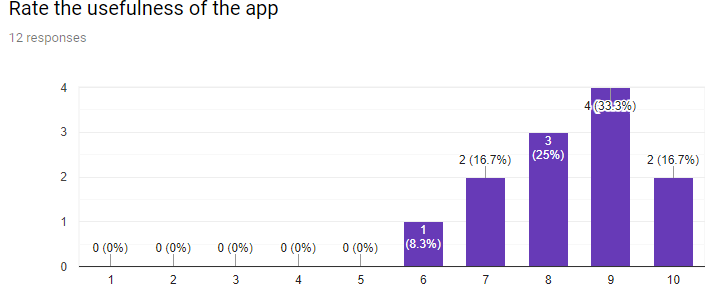
\includegraphics[width=.75\textwidth, keepaspectratio=true]{Img/Beta1}
\caption{Response beta testing 1}
\end{figure}
\vspace{-0.2cm}
\begin{figure}[h]
\centering
  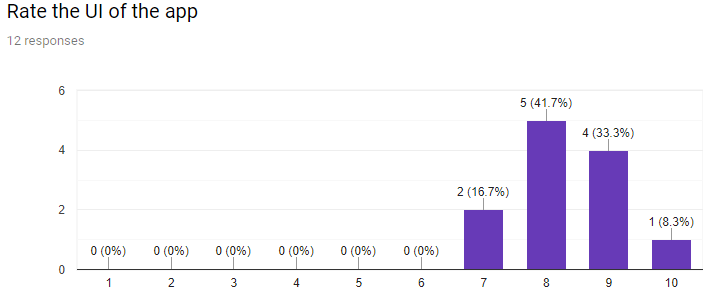
\includegraphics[width=.75\textwidth, keepaspectratio=true]{Img/Beta2}
\caption{Response beta testing 2}
\end{figure}
\vspace{-0.2cm}
\begin{figure}[h]
\centering
  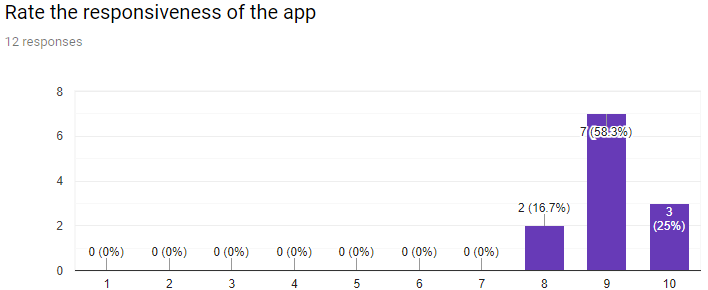
\includegraphics[width=.75\textwidth, keepaspectratio=true]{Img/Beta3}
\caption{Response beta testing 3}
\end{figure}
\clearpage
\begin{figure}[h]
\centering
  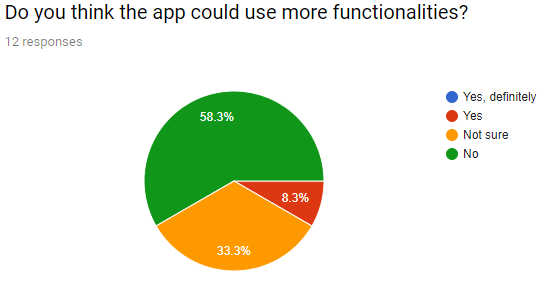
\includegraphics[width=.75\textwidth, keepaspectratio=true]{Img/Beta4}
\caption{Response beta testing 4}
\end{figure}
\begin{figure}[h]
\centering
  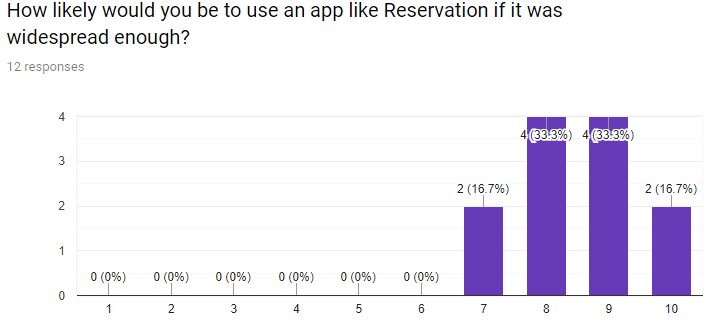
\includegraphics[width=.75\textwidth, keepaspectratio=true]{Img/Beta5}
\caption{Response beta testing 5}
\end{figure}

\noindent Even though the sample size was quite small the results of the testing can be considered quite satisfactory as a first testing by people that aren't familiar with software development.